\section{Aufbau und Durchführung}
\label{sec:Durchführung}
\subsection{Aufbau}
Der Aufbau der Apparatur findet sich in Abbildung \ref{fig:aufbau} wieder.
Zwischen den Polschuhen eines Elektronmagneten befindet sich eine Cadmium-Lampe.
Die Emissionslinien der Lampe werden senkrecht zur Feldrichtung kollimiert und in Richtung eines Geradsichtprismas gelenkt.
Das Prisma dient zur Aufspaltung in die Spektrallinien, welche schließlich auf einen Spalt abgebildet werden.
Am Spalt kann bestimmt werden mit welcher Linie gearbeitet werden soll.
Die Polarisationsrichtung der Strahlung wird mittels Polarisationsfilter eingestellt.
Eine Lummer-Gehrcke-Platte sorgt, durch Interferenzerscheinungen, für die Sichtbarkeit der Linienaufspaltung.
Mit einer Digitalkamera kann zum Schluss ein Bild von der Aufspaltung aufgenommen werden.
\begin{figure}
   \centering
    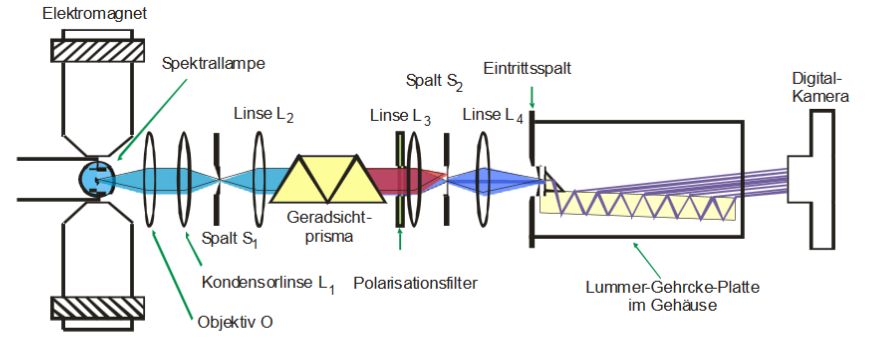
\includegraphics[width=0.8\textwidth]{aufbau.PNG}
    \caption{Der Aufbau der Apparatur.\cite{skript}}
    \label{fig:aufbau}
\end{figure}
\subsection{Durchführung}
Fotographiert wird für die rote Linie die
Aufspaltung, mit $\sigma$-Polarisation, bei ausgeschaltetem und angeschalteten Magnetfeld.
Für die blaue Linie wird zusätzlich die $\pi$-Polarisation berücksichtigt.
Zusätzlich wird eine Hysteresekurve des Magnetfeldes aufgenommen.
